\subsection{Motor modelling}\label{motormodelling}
In this section a model of a motor is depicted only as an electrical system, which delivers a rotational force called torque, \si{\tau_m}. The electrical model provides the motor's produced torque to the drivetrain which is further discussed in \secref{DriveTrain}.

%\subsubsection{Mechanical model}
%A mechanical model is formed to analyse the forces and inertias affecting the mechanical system, and to see how the system will react to stimuli.
%
%Newtons second law of motion for rotational systems yields:
%
%\begin{flalign}
%\eq{\tau_m(t)}{J_m \cdot \ddot{\theta}_m(t)} \unit{N\cdot m}
%\label{eq:mechanicalmodel}
%\end{flalign}
%\hspace{6mm} Where:\\
%\begin{tabular}{p{1cm}lll}
%& \si{J_m}             & is the motor's inertia                   &\unitWh{kg\cdot m^2}\\
%& \si{\ddot{\theta}_m} & is the angular acceleration in the motor &\unitWh{\frac{rad}{s^2}}
%\end{tabular}
%
%This law is applied to the mechanical model and visualized in \figref{fig:MotorMechanicalModel}. Furthermore it is necessary to consider the friction affecting the rotation of the motor when it is spinning. The friction is in the opposite direction of the applied rotational force torque, see \figref{fig:MotorMechanicalModel}.
%
%\begin{figure}[H]
%	\centering
%	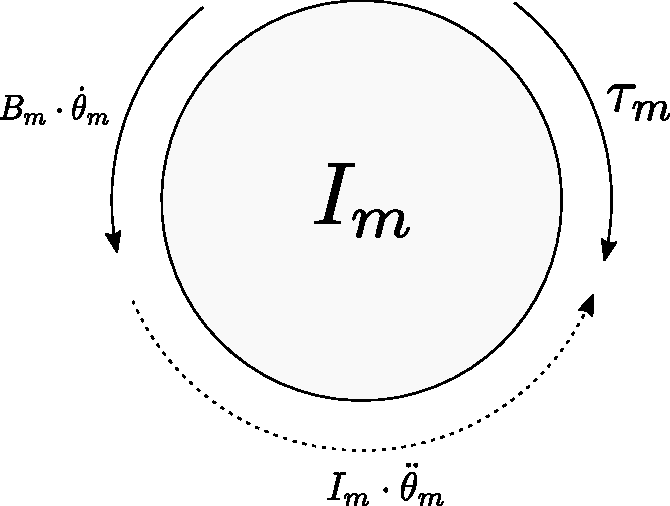
\includegraphics[scale=0.8]{figures/MotorMechanicalModel.pdf}
%	\caption{A free body diagram of the motor}
%	\label{fig:MotorMechanicalModel}
%\end{figure}
%
%From the figure an equation for the mechanical model can be derived.
%
%\begin{flalign}
%\eq{\tau_m(t)}{J_m \cdot \ddot{\theta}_m(t) + B \cdot \dot{\theta}_m(t)}\unit{N}
%\label{eq:mechaUnloadedMotor}
%\end{flalign}
%
%The equation is transferred into the frequency domain using the Laplace transform: 
%
%\begin{flalign}
%\eq{\tau_m(s)}{J_m(s) \cdot \omega_m \cdot s + B \cdot \omega_m}\unit{N}
%\label{eq:ThetadotforBlock}
%\end{flalign}
%
%The mechanical model of the motor has be derived. The mechanical contributions from the motor will be used to model the drivetrain. 
%
%Next step is to model the electrical part of the motor, and to find the motor's produced torque. 

\subsubsection{Electrical model}
The output needed from the motor's electrical model is the torque, \si{\tau_m}. To obtain the torque, the formula for translating the electrical current, \si{i_a}, to torque is utilized:

\begin{flalign}\centering
  \eq{\tau_m(t)}{K_t \cdot i_a} \unit{N \cdot m}
  \label{equ:motortorque}
\end{flalign}
\hspace{6mm} Where:\\
\begin{tabular}{p{1cm}lll}
& \si{\tau_m} & is the rotational force torque &\unitWh{N \cdot m} \\
& \si{i_a(t)} & is the electrical closed loop current &\unitWh{A}\\
& \si{K_t} & is the motor constant &\unitWh{N \cdot m \cdot A^{-1}}
\end{tabular}

An expression for the current, \si{i_a}, is required to derive a model for the electrical system. In \figref{fig:electricaldiagrammotor} an electrical diagram of the motor is displayed.

\begin{figure}[H]
\centering
	\begin{circuitikz}[american voltages]
		\draw
		
		% electromotive force 
		(0,0) to [short] (6,0)
		%to [sV, l=$e_b$] (6,2) %  voltage
		(6,0) to [V, l=$e_b$] (6,3)
		%to node[short]{}(6,2)

		%to node[short]{}(0,0)		 
		(0,0) to [V, l=$V_m$] (0,3) %  voltage

		
		%to [R, l=$Z_G$] (3,3) % generator impedance
		
		(0,3) to [R, l_=$R_a$, i>_=$i_a$] (3,3)	
		
		to [L, l_=$L_a$] (6,3); 
	\end{circuitikz}
  \caption{A electrical diagram of the motor}
  \label{fig:electricaldiagrammotor}
\end{figure}

By using Kirchoff voltage law on the closed loop, seen in \figref{fig:electricaldiagrammotor}, an expression including $i_a$ can be derived:

\begin{flalign}
\eq{U_a(t)}{R_a \cdot i_a(t) + L_a \cdot \frac{di_a}{dt} + e_b}\unit{V} 
\label{MotorClosedLoop}
\end{flalign}
\hspace{6mm} Where:\\
\begin{tabular}{p{1cm}lll}
& \si{U_a(t)} & is the supply voltage                       &\unitWh{V} \\
& \si{R_a}    & is the internal resistance in the motor     &\unitWh{\Omega}\\
& \si{L_a}    & is the inductance in the motor              &\unitWh{H} \\
& \si{e_b}    & is the electromotive force, also called EMF &\unitWh{V} \\
\end{tabular}

The electromotive force, \si{e_b}, is equivalent to:

\begin{flalign}
\eq{e_b}{K_e \cdot \dot{\theta}_m(t)}\unit{V} 
\end{flalign}
\hspace{6mm} Where:\\
\begin{tabular}{p{1cm}lll}
& \si{K_e}            & is the electromotive constant        &\unitWh{Wb} \\
& \si{\dot{\theta}_m} & is the angular velocity in the motor &\unitWh{rad \cdot s^{-1}} \\
\end{tabular}

The equivalent for the electromotive force is substituted into \eqref{MotorClosedLoop}.

\begin{flalign}
\eq{U_a(t)}{R_a \cdot i_a(t) + L_a \cdot \frac{di_a}{dt} + K_e \cdot \dot{\theta}_m(t)}&
\end{flalign}

The Laplace transform is applied to the derived equation:

\begin{flalign}
\eq{U_a(s)}{R_a \cdot i_a(s) + L_a \cdot s \cdot i_a(s) + K_e \cdot \omega_m(s)}&
\end{flalign}

The equation is solved for \si{i_a}:

\begin{flalign}
\eq{i_a(s)}{\frac{U_a(s) - K_e \cdot \omega_m(s)}{L_a \cdot s + R_a}}&
\end{flalign}

By substituting the derived equation for $i_a$ into \eqref{equ:motortorque}, a new expression for the motor's torque is derived. 

\begin{flalign}
\eq{\tau_m}{K_t \cdot i_a(s)}&\nonumber\\
\eq{\tau_m}{K_t \cdot \frac{U_a(s) - K_e \cdot \omega_m(s)}{L_a \cdot s + R_a}}
  \label{eq:Totaltorquewithcurrentexpression}
\end{flalign}

By dividing with the voltage applied to the motor, $U_a$, a transfer function can be established:

\begin{flalign}
\eq{\frac{\tau_m}{U_a(s) - K_e \cdot \omega_m(s)}}{\frac{K_t}{L_a \cdot s + R_a}}&
  \label{eq:TotaltorquewithcurrentexpressionTransferFunction}
\end{flalign}

A transfer function for the electrical model relative to the motor's torque has been derived. Thus enabling setting up calculations for the vehicle's drivetrain.